\setcounter{section}{4}
\setcounter{subsection}{5}
\setcounter{subsubsection}{3}
\setcounter{figure}{11}
\setcounter{equation}{38}

\paragraph{Kopplung zwischen Rotation und Schwingung}
	Experimentellen Hinweisen zufolge rücken im P-Zweig mit zunehmenden $J$ die Linien auseinander und im R-Zweig zueinander. Die Ursache dessen ist, dass Schwingungen im Mittel 1000 mal schneller als die Rotationen sind. Die Rotation sieht somit den über die Schwingung gemittelten Kernabstand $\left<R \right>$, welcher mit zunehmender Quantenzahl $ \nu$ steigt. Es gilt
	$$
	\left< \Theta( \nu +1) \right> > \left< \Theta ( \nu) \right> > \Theta_{\mathrm{e}} 
	$$ 
	mit $ B \sim 1 / \Theta$.\\
	Die korrigierten Terme lauten somit
	$$
	\begin{aligned}
		B_{ \nu} &= B_{\mathrm{e}} - \alpha \left( \nu + \frac{1}{2} \right)  + \text{Glieder höherer Ordnung}, \\
		D_{ \nu} &= D_{\mathrm{e}} - \beta \left( \nu + \frac{1}{2} \right) +  \text{Glieder höherer Ordnung},\\
	\end{aligned}
	$$ 
	wobei $ \alpha$ und $ \beta$ molekülspezifische Konstanten sind mit $ \alpha \ll B_{\mathrm{e}}$, $ \beta \ll D_{\mathrm{e}}$.\\

	Nun betrachten wir die Schwingungs- und Rotationsdehnung. Für die Rotationsenergie gilt
	\begin{equation}
		\label{eq:4.39}
		E_{ \nu, J} = \hbar \omega_{\mathrm{e}} \left( \nu + \frac{1}{2} \right) - X_{\mathrm{e}} \hbar \omega_{\mathrm{e}} \left( \nu + \frac{1}{2} \right) ^2 + \mathrm{h}\mathrm{c} B_{ \nu} J(J+1) - \mathrm{h} \mathrm{c} D_{ \nu} J^2 (J+1)^2.
	\end{equation}
	\autoref{fig:vl10_grundschwingungen_CO} zeigt das korrigierte Energiespektrum am Beispiel von Kohlenstoffmonoxid \ce{CO}.

	\begin{figure}[H]
		\centering
		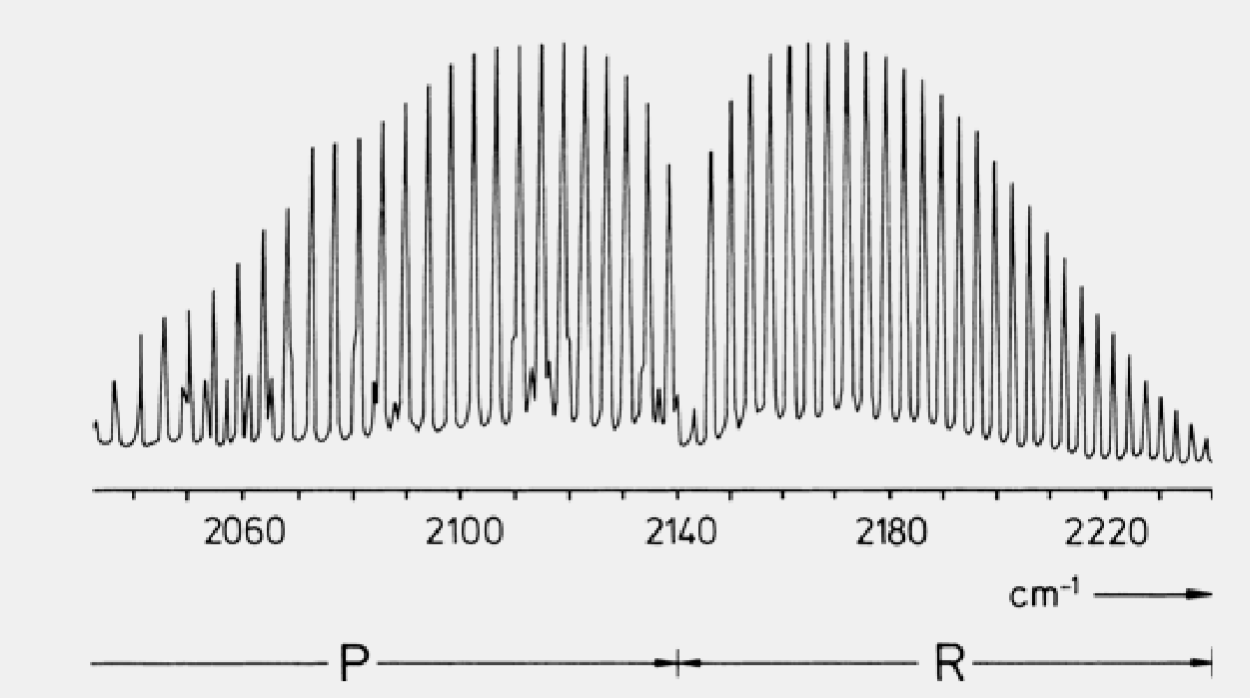
\includegraphics[width=0.6\linewidth]{figures/vl10/grundschwingungen_CO.png}
		\caption{Flügelförmiges Schwingungsspektrum des \ce{CO}-Moleküls \cite{Haken_Wolf_2006}. Der linke Flügel ist der P-Zweig, der rechte der R-Zweig.}
		\label{fig:vl10_grundschwingungen_CO}
	\end{figure}

	\subsubsection{Schwingungen vielatomiger Moleküle}
	\paragraph{Wiederholung Normalschwingungen}
	Bei einer Normalschwingung handelt es sich um ein Schwingen der Massenpunkte mit gleicher Frequenz und fester Phasenbeziehung. Alle andere Schwingungen sind Linearkombinationen der Normalschwingungen.
	Ein Beispiel dafür ist das gekoppelte Pendel. Deren Normalschwingungen sind die symmetrische (\autoref{fig:vl10_fadenpendel_symmetrisch}) und die antisymmetrische Mode (\autoref{fig:vl10_fadenpendel_antisymmetrisch}).\\

	\begin{minipage}{0.46\linewidth}
		\centering
		\includegraphics[width=0.5\textwidth]{./figures/VL10_Abbildung_2.tikz}
		\captionof{figure}{Symmetrische Mode des gekoppelten Pendels mit Pendelpositionen $x_1$, $x_2$ und der Bedingung $x_1=x_2$.}
		\label{fig:vl10_fadenpendel_symmetrisch}
	\end{minipage}
	\hspace{0.07\linewidth}
	\begin{minipage}{0.46\linewidth}
		\centering
		\includegraphics[width=0.5\textwidth]{./figures/VL10_Abbildung_3.tikz}
		\captionof{figure}{Antisymmetrische Mode des gekoppelten Pendels mit Pendelpositionen $x_1$, $x_2$ und der Bedingung $x_1=-x_2$.}
		\label{fig:vl10_fadenpendel_antisymmetrisch}
	\end{minipage}

	Die Anzahl $f$ der Normalschwingungen eines Systems ist die Zahl der Freiheitsgrade, die noch nicht für andere Bewegungen verbraucht sind. Bei $N$ Massenpunkten gibt es $3N$ Freiheitsgrade, wovon 3 Freiheitsgrade an die Translation des Schwerpunkts und 3 weitere an Rotation um den Schwerpunkt abgehen (2 bei linearen Molekülen).\\

	\begin{important}
		Die Anzahl $f$ der Normalschwingungen eines mehratomigen Moleküls ist\\
		\hspace{-1.5cm}\begin{tabular}{ll}
			allgemein: & $f=3N-6$\\
			bei linearen Molekülen: & $f=3N-5$
		\end{tabular} 
	\end{important}

\paragraph{Beispiel 1: \ce{HCl}}
	\ce{HCl} ist zweitatomig und linear, also $N =2 $, womit ${f = 3\cdot 2 - 5 = 1}$. Dieser Freiheitsgrad entspricht der Streckschwingung.

\paragraph{Beispiel 2: \ce{CO2}} 
	Für dreiatomige lineare Moleküle wie \ce{CO2} gilt $f = 3\cdot 3 -5 = 4$. Die Normalschwingungen sind in \autoref{fig:vl10_normalschwingungen_CO2} dargestellt.
	\begin{figure}[H]
		\centering
		\includegraphics[width=0.7\textwidth]{./figures/VL10_Abbildung_4.tikz}
		\caption{Normalschwingungen von Kohlenstoffdioxid \ce{CO2}.}
		\label{fig:vl10_normalschwingungen_CO2}
	\end{figure}
	Die dargestellten Moden des Kohlenstoffdioxids sind 
	\begin{itemize}
		\item{Links:} symmetrische Streckschwingung. Sie ist IR-inaktiv, da $\frac{\partial\vec p}{\partial r}=0$ mit Wellenzahl $\overline\nu_1=\SI{1337}{\per\centi\meter}$.
		\item{Mitte:} unsymmetrische Streckschwingung. Sie ist IR-aktiv mit Wellenzahl $\overline\nu_2=\SI{2349}{\per\centi\meter}$.
		\item Rechts: zwei Knickschwingungen in schwarz und blau. Sie sind IR-aktiv mit Wellenzahl $\overline\nu_3=\overline\nu_4=\SI{667}{\per\centi\meter}$.
	\end{itemize}

Generell sind die Frequenzen von Streckschwingungen größer als diejenigen von Biegeschwingungen.

\paragraph{Beispiel 3: \ce{H2O}}
	Für dreiatomige gewinkelte Moleküle wie \ce{H2O} gilt $f = 3\cdot 3 - 6 = 3$. Die Schwingungsmoden des Wassermoleküls sind in \autoref{fig:vl10_normalschwingungen_H20} dargestellt.\\
	\begin{figure}[H]
		\centering
		\includegraphics[width=0.7\textwidth]{./figures/VL10_Abbildung_5.tikz}
		\caption{Normalschwingungen von Wasser \ce{H2O}.}
		\label{fig:vl10_normalschwingungen_H20}
	\end{figure}
	Alle Moden von Wasser sind IR-aktiv wegen der freien Elektronenpaare am Sauerstoffatom. Die dargestellten Moden von \ce{H2O} sind 
	\begin{itemize}
		\item{Links:} symmetrische Streckschwingung mit Wellenzahl $\overline\nu_1=\SI{3652}{\per\centi\meter}$.
		\item{Mitte:} unsymmetrische Streckschwingung mit Wellenzahl $\overline\nu_2=\SI{3756}{\per\centi\meter}$.
		\item Rechts: Knickschwingung mit Wellenzahl $\overline\nu_3=\SI{1595}{\per\centi\meter}$.
	\end{itemize}

	Die Anharmonizität im Kraftgesetz führt zur Kopplung der Normalschwingungen. Daher kommt es zu
	\begin{itemize}
		\item Obertönen $2 \nu_1$, $3 \nu_1$, \ldots
		\item Kombinationsschwingungen, also der Summe oder Differenz von Schwingungen
			$$
			\nu_1 + \nu_2, \quad \nu_2 - \nu_1, \ldots
			$$ 
	\end{itemize}

\subsubsection{Anwendungen der Schwingungsspektroskopie}
	Schwingungsspektroskopie wird verwendet, um Moleküle oder Molekülteile zu identifizieren. Dazu wird z.B. die Valenzschwingung betrachtet, also die Schwingung einer Verbindungsachse zwischen Atomen. So können verschiedene Bindungen identifiziert werden, bspw.
	\begin{itemize}
		\item \ce{C-H} hat eine Valenzschwingung mit $\SI{2850}{\centi \meter ^{-1}}$ bis $\SI{3000}{\centi \meter ^{-1}}$
		\item \ce{C-C} hat eine Valenzschwingung mit $\SI{700}{\centi \meter ^{-1}}$ bis $\SI{1250}{\centi \meter ^{-1}}$
		\item \ce{C=C} hat eine Valenzschwingung mit $\SI{1600}{\centi \meter ^{-1}}$ bis $\SI{1700}{\centi \meter ^{-1}}$
	\end{itemize}

	\subsubsection{Infrarot-Laser}
	In einem Infrarot-Laser, auch CO2-Laser genannt, befindet sich ein Gasgemisch aus Stickstoff \ce{N2}, Kohlenstoffdioxid \ce{CO2} und Helium \ce{He}.\\[2em]
	\begin{minipage}{0.45\linewidth}
		\centering
		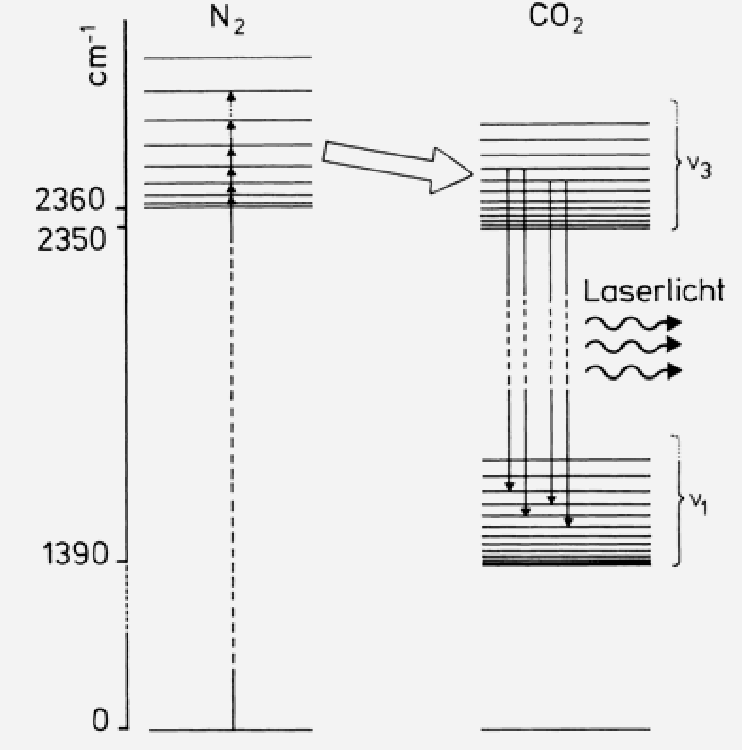
\includegraphics[width=6cm]{figures/vl10/CO2_laser.png}
		\captionof{figure}{Termschema der Prozesse im Infrarot-Laser \cite{Haken_Wolf_2006}.}
		\label{fig:vl10_CO2_laser}
	\end{minipage}
	\hspace{0.05\linewidth}
	\begin{minipage}{0.5\linewidth}
		\autoref{fig:vl10_CO2_laser} zeigt die Prozesse eines Infrarot-Lasers im Termschema. 
		Elektronen werden aus dem Grundzustand in einen erhöhten Zustand im Stickstoff angeregt.
		Da \ce{N2} und \ce{CO2} nahezu resonant sind, können die Elektronen von dort in den angeregten Zustand $\nu=3$ des Kohlenstoffdioxids übergehen.
		Dort fallen sie in den $\nu=1$ Zustand des \ce{CO2} und emittieren dabei Laserlicht mit Wellenlänge \SI{10,6}{\micro\meter}, bzw. Wellenzahl $\sim\SI{1000}{\per\centi\meter}$.
		Von dort fallen die Elektronen durch Stöße mit Helium wieder in den Grundzustand.
	\end{minipage}\\[1em]
	Der CO2-Laser kann sehr hohe Leistungen aufbringen. Deshalb wird er in der Industrie sehr viel verwendet, u.A. um Metalle zu zerschneiden.

\subsubsection{Mikrowellen-MASER}
	MASER steht abgekürzt für Microwave Amplification by Stimulated Emission of Radiation. Er wurde im Jahr 1955 von Gordon, Zeiger und Townes entwickelt.

	Das zugrundeliegende Phänomen ist die Inversionsschwingung von Ammoniak \ce{NH3}, wie sie in \autoref{fig:vl10_ammoniak_inversionsschwingung} dargestellt ist.

	\begin{figure}[H]
		\centering
		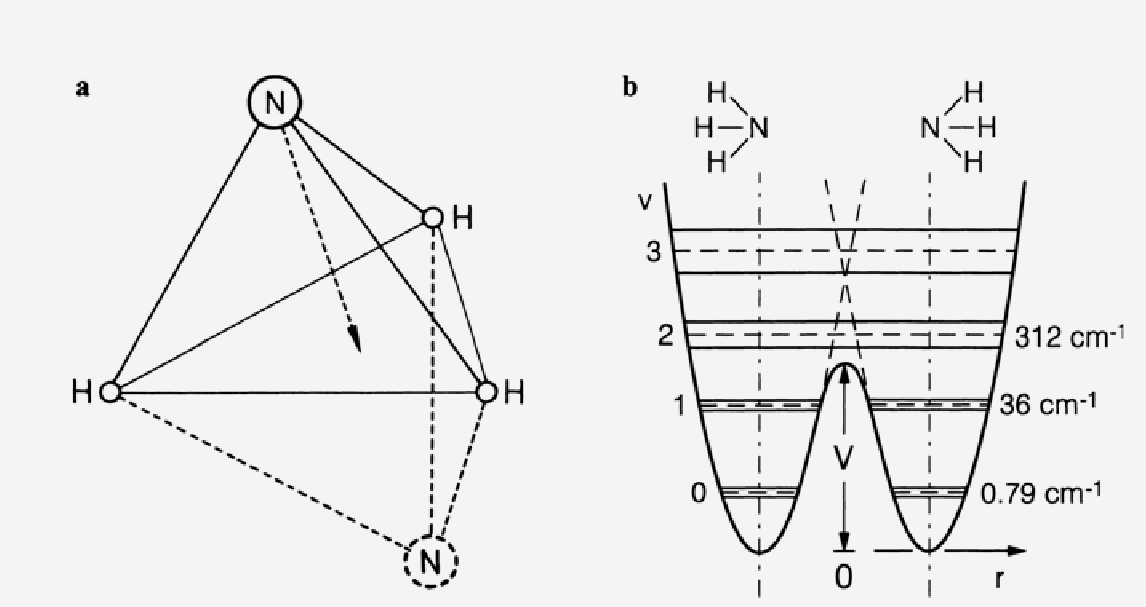
\includegraphics[width=0.8\linewidth]{figures/vl10/maser_stickstoff_doppelmulde.png}
		\caption{Links: Ammoniakmolekül.
			Das Stickstoffatom kann sich über und unter der Ebene aufhalten, welche von den Wasserstoffatomen aufgespannt wird.\\
			Rechts: Daher kann es in einem Doppelmuldenpotential $V(r)$ modelliert werden, welches vom Abstand $r$ des Stickstoff zur Wasserstoffebene abhängt.
		}
		\label{fig:vl10_ammoniak_inversionsschwingung}
	\end{figure}
	Durch den Potentialwall der Höhe $V$ kommt es zur Inversionsaufspaltung in eine symmetrische Mode $\varphi_\mathrm s = N(\phi_1+\phi_2)$ und eine antisymmetrische Mode $\varphi_\mathrm a = N(\phi_1-\phi_2)$.
	Die Wellenfunktionen $\phi_i$ stellen dabei das Teilchen in jeweils einer der beiden Mulden dar.
	Die beiden Moden haben folgende Eigenschaften:
	\begin{enumerate}
		\item zwischen $ \varphi_{a}$ und $ \varphi_{s}$ sind elektromagnetische Übergänge erlaubt
		\item $ \varphi_{a}$ und $ \varphi_{s}$ haben $ \Vec{p}=0$ wegen der Inversionsschwingung. 
			Würde man den Tunneleffekt vernachlässigen, wäre $\Vec{p} \neq 0$ aufgrund der Partialladungsverschiebung im Molekül.
		\item im $\Vec{E}$-Feld kommt es zum Stark-Effekt, also der Aufspaltung der Schwingungsniveaus gemäß \autoref{fig:vl10_stark_effekt}.
			\begin{figure}[H]
				\centering
				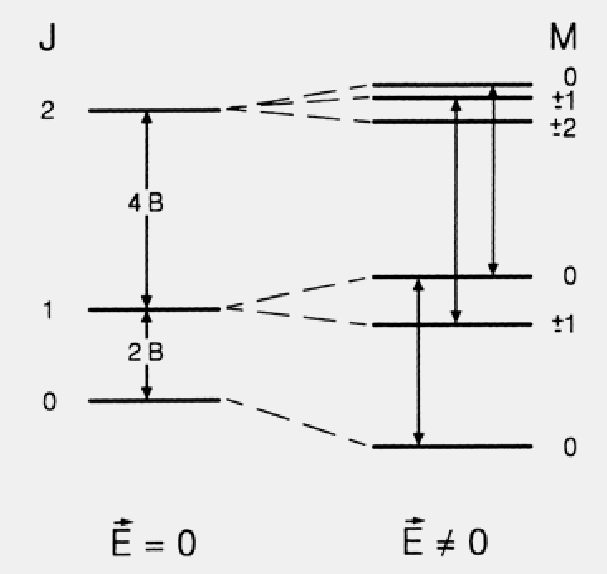
\includegraphics[width=0.35\linewidth]{figures/vl10/stark_effekt.png}
				\caption{Beim Stark-Effekt kommt es zu Aufspaltung der Schwingungsniveaus.}
				\label{fig:vl10_stark_effekt}
			\end{figure}
		\item im inhomogenen Feld läuft $ \varphi_{s} $ in das starke Feld, da es energetisch günstiger liegt. $ \varphi_{a} $ läuft in das schwache Feld.
	\end{enumerate}

	Es ist $ \Delta \ll \mathrm{k}_{\mathrm{B}} T$. Dadurch wird Trennung von $\varphi_a$ und $\varphi_s$ möglich.

	\autoref{fig:vl10_NH3_maser} zeigt den Aufbau eines Mikrowellen-Masers. 
	Der Stark-Effekt ermöglicht die Aufspaltung des \ce{NH3}-Strahles aus dem Ofen, sodass nur die antisymmetrischen Teilchen $\varphi_\mathrm a$ in den Mikrowellen-Resonator kommen.
	Dort fallen sie in den symmetrischen Zustand $\varphi_\mathrm s$, der energetisch niedrigier liegt und emittieren dabei Mikrowellen-Strahlung.

	\begin{figure}[H]
		\centering
		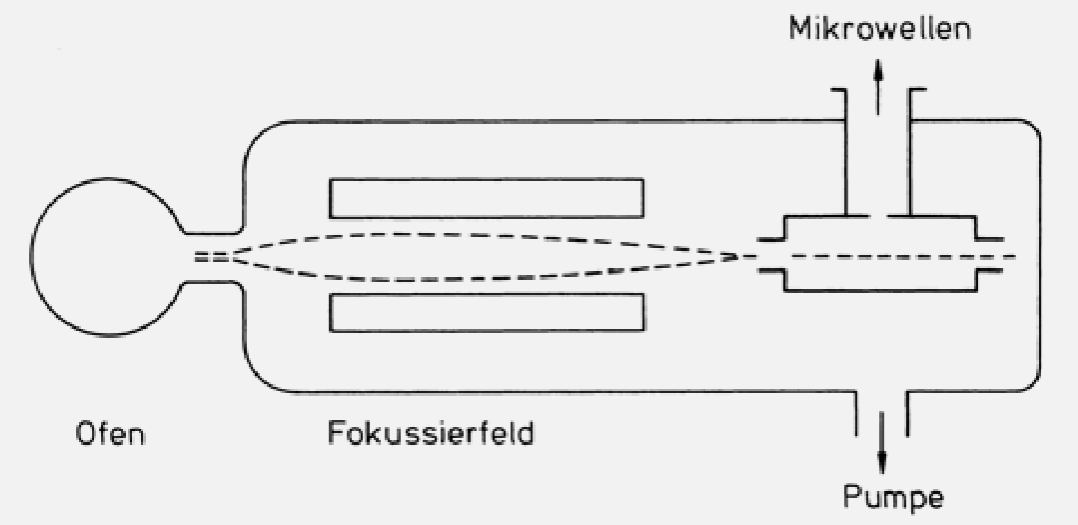
\includegraphics[width=0.8\linewidth]{figures/vl10/NH3_maser.png}
		\caption{Schematischer Aufbau eines \ce{NH3}-Masers.}
		\label{fig:vl10_NH3_maser}
	\end{figure}

	Der \ce{NH3}-Maser ist somit ein Zwei-Niveau-Maser. 
	Die Energiebreite ist $\frac{\Delta\nu}{\nu}=\SI{10e10}{}$, also hat der Maser ein sehr schmales Frequenzspektrum.